\begin{tikzpicture}[scale=0.5,>=stealth]
\scriptsize
\fill [gray!20] (-2.5,7.5) -- (-2.5,3.5) -- (2,3.5) -- (2,5.5) -- (5,5.5) -- (5,7.5) -- cycle;
\node at (1,7) [label=right:{$F\!=$Display}] {};
\node at (1,6.5) [label=right:{$F_1\!=$Monitor}] {};
\node at (1,6) [label=right:{$F_2\!=$Computer}] {};
\drawFluent{-2}{7}{0.4};\node at (-1.75,7) [label=right:Fluent] {};
\drawAction{-2}{6}{0.4};\node at (-1.75,6) [label=right:Action] {};
\drawInertialAction{-2}{5}{0.4};\node at (-1.75,5) [label=right:Inertial Action] {};
\drawTransitNP{-2}{4}{0.4};\node at (-1.75,4) [label=right:Fluent Transit] {};
%
\draw [->,red!50] (1,0) -- (1.5,1.65);
\draw [->,red!50] (2,0) -- (1.5,1.65);
\draw [->,red!50] (4,0) -- (4.5,1.65);
\draw [->,red!50] (5,0) -- (4.5,1.65);
\draw [->,very thick,red] (7,0) -- (7.5,1.65);
\draw [->,very thick,red] (8,0) -- (7.5,1.65);
\draw [->,red!50] (1.5,2) -- (4.5,3.75);
\draw [->,red!50] (4.5,2) -- (4.5,3.75);
\draw [->,very thick,red] (7.5,2) -- (4.5,3.75);
\draw [->,very thick,red] (10.5,2) -- (11.25,3.75);
\draw [->,red!50] (12,2) -- (11.25,3.75);
\draw [->,very thick,red] (4.5,4) -- (7.875,5.75);
\draw [->,very thick,red] (11.25,4) -- (7.875,5.75);
%
\draw [very thick,red,shift={(7.875,5.75)}] (0,0)+(-150:6mm) arc (-150:-30:6mm);
\draw [red!50,shift={(1.5,1.65)}] (0,0)+(-105:6mm) arc (-105:-75:6mm);
\draw [red!50,shift={(4.5,1.65)}] (0,0)+(-105:6mm) arc (-105:-75:6mm);
\draw [very thick,red,shift={(7.5,1.65)}] (0,0)+(-105:6mm) arc (-105:-75:6mm);
%
\drawFluent{1}{0}{0.4};\node at (1,-1) [] {\parbox{1.5cm}{\centering $F_2(t\!-\!1)\!=$\\AWAKE}};
\drawInertialAction{2}{0}{0.4};
\drawFluent{4}{0}{0.4};\node at (4,-1) [] {\parbox{1.5cm}{\centering $F_2(t\!-\!1)\!=$\\ASLEEP}};
\drawAction{5}{0}{0.4};
\drawFluent{7}{0}{0.4};\node at (7,-1) [] {\parbox{1.5cm}{\centering $F_2(t\!-\!1)\!=$\\ASLEEP}};
\drawAction{8}{0}{0.4};
\drawTransitPP{1.5}{2}{0.4};
\drawTransitNP{4.5}{2}{0.4};
\drawTransitNP{7.5}{2}{0.4};
\drawTransitPP{10.5}{2}{0.4};
\drawTransitNP{12}{2}{0.4};
\drawFluent{4.5}{4}{0.4};\node at (4.75,4) [label=right:{$F_2(t)\!=$AWAKE}] {};
\drawFluent{11.25}{4}{0.4};\node at (11.5,4) [label=right:{\parbox{1cm}{$F_1(t)\!=$\\POWERED}}] {};
\drawHollowFluent{7.875}{6}{0.4}\node at (8.125,6) [label=right:{$F(t)\!=$ON}] {};
\draw [dashed,thick] (5.75,-2.75) [out=90,in=-45] to (5.25,-0.25);
\draw [dashed,thick] (8.75,-2.75) [out=90,in=-45] to (8.25,-0.25);
\node at (5.75,-2.75) [] {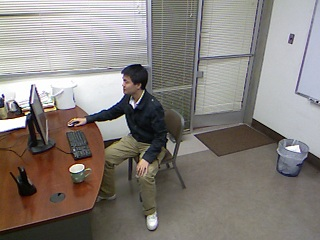
\includegraphics[width=.5in]{185}};
\node at (8.75,-2.75) [] {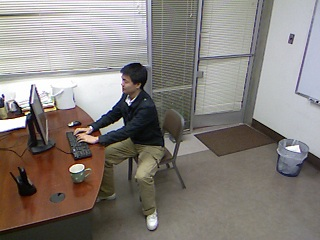
\includegraphics[width=.5in]{275}};
%
\node at (7.875,7) [] {\bf (a) Causal-AOG};
\node at (20,7) [] {\bf (b) Causal-PG};
%
\draw [->,thick] (18,5) -- (24,5);
\draw [thick,cyan] (16,2.75) -- (20,2.75);
\draw [thick,cyan] (20,3.25) -- (24,3.25);
\draw [thick,cyan] (16,0.75) -- (20,0.75);
\draw [thick,cyan] (20,1.25) -- (24,1.25);
\draw [thick,cyan] (16,-0.75) -- (24,-0.75);
\drawAction{18}{5}{0.4};
\node at (20,5.75) [] {Use Keyboard$(t\!-\!1,t_2)$};
\drawFluent{18}{3}{0.4};\drawTransitNP{20}{3}{0.4};\drawFluent{22}{3}{0.4};
\node at (18,2.25) [] {$F_2(t\!-\!1)\!=$ASLEEP};
\node at (22,3.75) [] {$F_2(t)\!=$AWAKE};
\drawFluent{18}{1}{0.4};\drawTransitNP{20}{1}{0.4};\drawFluent{22}{1}{0.4};
\node at (18,0.25) [] {$F(t\!-\!1)\!=$OFF};
\node at (22,1.75) [] {$F(t)\!=$ON};
\drawFluent{18}{-1}{0.4};\drawTransitPP{20}{-1}{0.4};\drawFluent{22}{-1}{0.4};
\node at (18,-1.75) [] {\parbox{1.5cm}{\centering $F_1(t\!-\!1)\!=$\\POWERED}};
\node at (22,-1.75) [] {\parbox{1.5cm}{\centering $F_1(t)\!=$\\POWERED}};
\draw [->,thick] (16,-3) -- (24,-3);\node at (24,-3) [label=below:Time] {};
\draw (18,-2.75) -- (18,-3.25);\node at (18,-3) [label=below:$t\!-\!1$] {};
\draw (22,-2.75) -- (22,-3.25);\node at (22,-3) [label=below:$t$] {};
\node at (15.5,5) [] {\begin{sideways}\parbox{1cm}{\centering Agent\\Action}\end{sideways}};
\node at (15.5,3) [] {\begin{sideways}Computer\end{sideways}};
\node at (15.5,1) [] {\begin{sideways}Display\end{sideways}};
\node at (15.5,-1) [] {\begin{sideways}Monitor\end{sideways}};
%
\draw [->,very thick,red] (18.4,5) -- (19.75,3.25);
\draw [->,very thick,red] (18.25,3) -- (19.6,3);
\draw [->,very thick,red] (20.4,3) -- (21.75,3);
\draw [->,very thick,red] (22,2.75) -- (22,2);
\draw [->,very thick,red] (22,-0.5) -- (22,0.75);
\draw [->,very thick,red] (18.25,-1) -- (19.6,-1);
\draw [->,very thick,red] (20.4,-1) -- (21.75,-1);
\end{tikzpicture}